\documentclass{standalone}
\usepackage{tikz}
\usepackage{pgfplots}
\pgfplotsset{width=32cm,height=18cm,compat=1.3}
\pgfplotsset{every tick label/.append style={font=\Huge}}
\usepackage{filecontents}

\usetikzlibrary{patterns}

\definecolor{citrine}{rgb}{0.89, 0.82, 0.04}

\begin{document}
	\centering
		\vspace{1.5em}
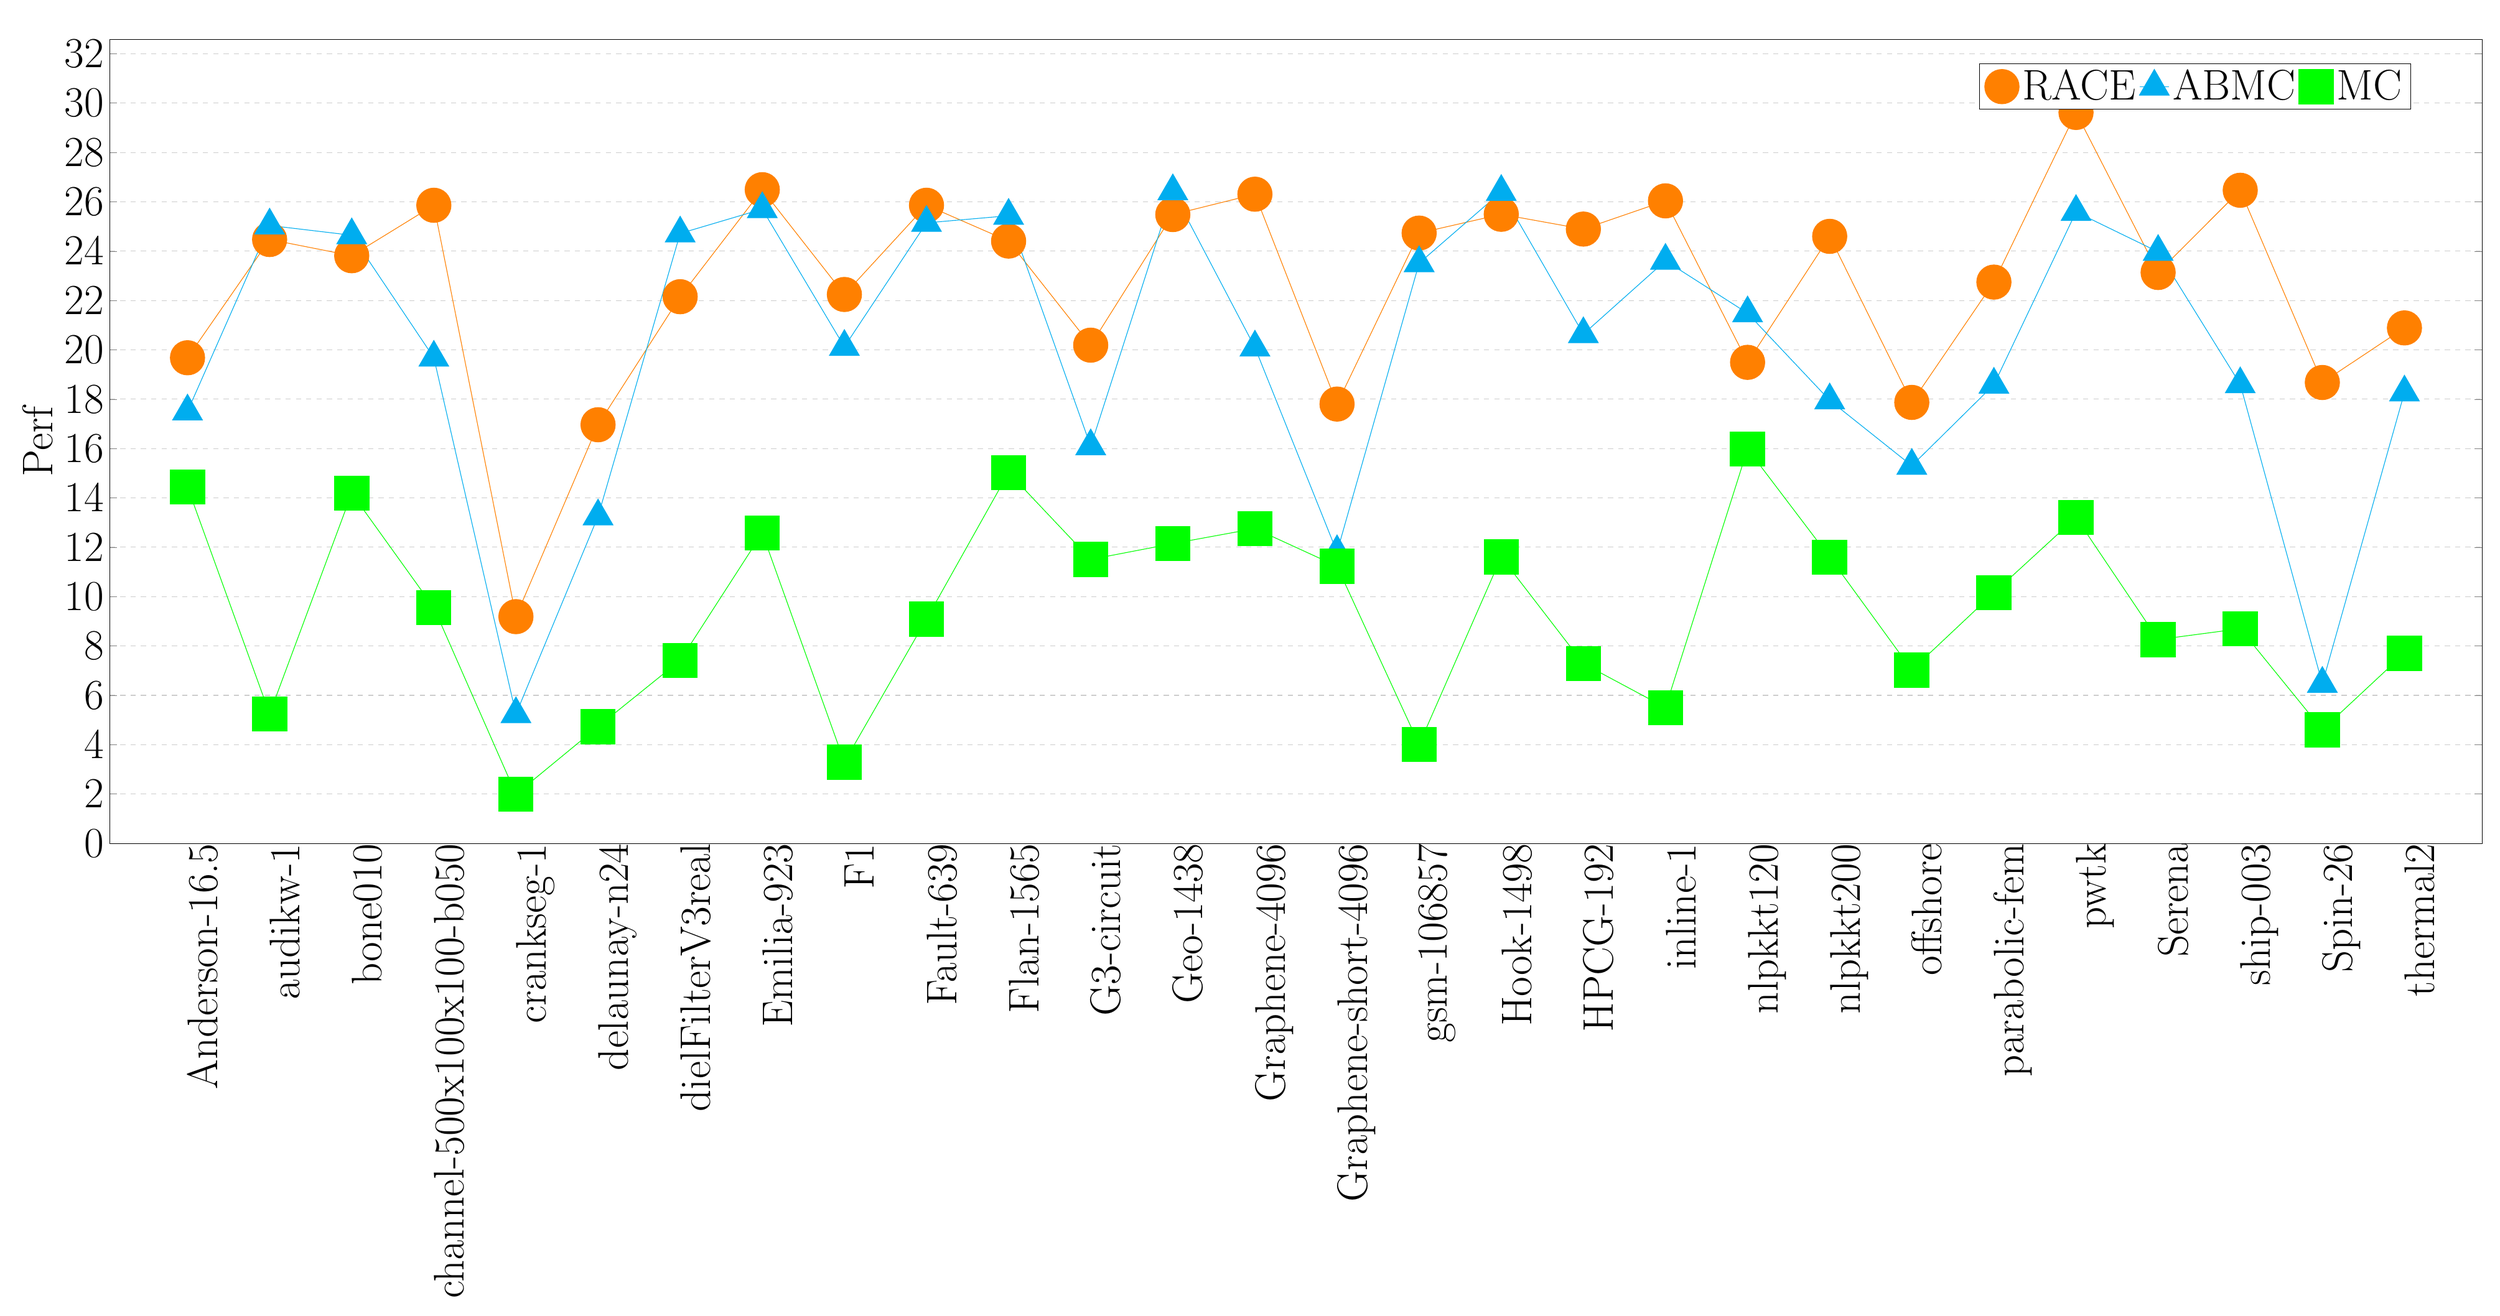
\begin{tikzpicture}
		%	\node at (13.25,15) {\LARGE{}};
			\begin{axis}[
		%	xmin=0.25, xmax=7.25,
			ymin=0, %ymax=3.25,
			xtick={1, 2, 3, 4, 5, 6, 7, 8, 9, 10, 11, 12, 13, 14, 15, 16, 17, 18, 19, 20, 21, 22, 23, 24, 25, 26, 27, 28},
		%	ytick={0,0.5,1,1.5,2,2.5,3},
			xticklabels={Anderson-16.5, audikw-1, bone010, channel-500x100x100-b050, crankseg-1, delaunay-n24, dielFilterV3real, Emilia-923, F1, Fault-639, Flan-1565, G3-circuit, Geo-1438, Graphene-4096, Graphene-short-4096, gsm-106857, Hook-1498, HPCG-192, inline-1, nlpkkt120, nlpkkt200, offshore, parabolic-fem, pwtk, Serena, ship-003, Spin-26, thermal2},
			width  = 50cm,
			height = 18cm,
			major x tick style = transparent,
			%	minor ytick={1, 5, 10, 15, 20, 25, 30 ,35,40},
			grid = minor,	
			%add_bar_commands
			ymajorgrids = true,
			grid style={dashed, gray!40},
			ylabel = {\Huge{Perf}},
		%	symbolic x coords={Graphene-2048-2048, Graphene-4096-4096, Spin-24-24-24},
			x tick label style={rotate=90, anchor=north east, inner sep=0mm, font={\Huge}},
			tick label style={font={\Huge}},
			scaled y ticks = false,
			enlarge x limits=0.035,
			legend cell align=left,
			legend style={font=\Huge},
			legend columns=-1,
			legend style={
				%at={(1,1.05)},
				%anchor=south east,
				%column sep=1ex,
				legend pos=north east
			},
			%spl_legend_code
			title= {\Huge\scalebox{1.5}{{}}}
			]

\addplot[mark=*, mark size=10pt, mark options={orange}, draw=orange ] plot coordinates{(1,19.678338) (2,24.470638) (3,23.813569) (4,25.858192) (5,9.188028) (6,16.964026) (7,22.152597) (8,26.490050) (9,22.243093) (10,25.859193) (11,24.406704) (12,20.189379) (13,25.481092) (14,26.306260) (15,17.802001) (16,24.731023) (17,25.492494) (18,24.893000) (19,26.036429) (20,19.492790) (21,24.598421) (22,17.869342) (23,22.744309) (24,29.619693) (25,23.134373) (26,26.465952) (27,18.676146) (28,20.888076)};
\addplot[mark=triangle*, mark size=10pt, mark options={cyan}, draw=cyan ] plot coordinates{(1,17.504669) (2,25.039542) (3,24.643671) (4,19.682763) (5,5.237748) (6,13.253567) (7,24.716414) (8,25.701974) (9,20.122238) (10,25.145408) (11,25.433920) (12,16.095095) (13,26.428093) (14,20.095991) (15,11.802042) (16,23.512788) (17,26.400655) (18,20.636315) (19,23.611138) (20,21.481489) (21,17.954247) (22,15.303070) (23,18.587763) (24,25.587634) (25,23.969977) (26,18.606680) (27,6.466911) (28,18.272815)};
\addplot[mark=square*, mark size=10pt, mark options={green}, draw=green ] plot coordinates{(1,14.443050) (2,5.250340) (3,14.188078) (4,9.552907) (5,1.991533) (6,4.731314) (7,7.415697) (8,12.578046) (9,3.295957) (10,9.090876) (11,15.026665) (12,11.507194) (13,12.147435) (14,12.757724) (15,11.231440) (16,4.007839) (17,11.603119) (18,7.284023) (19,5.502482) (20,15.984644) (21,11.597878) (22,7.025583) (23,10.155564) (24,13.208866) (25,8.258869) (26,8.698461) (27,4.604878) (28,7.705833)};
	%addplot cmd

	\legend{RACE, ABMC, MC}

	\end{axis}			
\end{tikzpicture}

\end{document}

